\chapter{Epimetheus}
\label{cap:epimetheus}

Il progetto Epimetheus nasce con l'obiettivo di migliorare le previsioni sullo stato di salute dei pazienti sottoposti a interventi chirurgici all'anca o al ginocchio. Questo prodotto si pone nel contesto di strumenti di supporto alle decisioni mediche, utilizzando un complesso sistema di machine learning per elaborare predizioni a partire dai dati PROM (Patient-Reported Outcome Measures).\\
L'adozione di Epimetheus è prevista presso l'IRCCS Istituto Ortopedico Galeazzi (IOG) di Milano, un'importante struttura sanitaria universitaria specializzata nella diagnosi e nel trattamento dei disturbi muscolo-scheletrici. Presso lo IOG vengono eseguiti annualmente quasi 5000 interventi chirurgici, con una prevalenza di artroplastiche dell'anca e del ginocchio, oltre a numerose procedure relative alla colonna vertebrale.\\
Epimetheus mira a rispondere a una necessità cruciale: migliorare la qualità delle previsioni cliniche post-operatorie. Attualmente, circa il 39\% degli interventi chirurgici alla colonna vertebrale presso lo IOG non raggiunge un miglioramento clinicamente significativo, e il 22\% di questi è associato a esiti negativi. Queste cifre sono dovute, in parte, al fatto che l'istituto Galeazzi è una struttura terziaria che accoglie i casi più complessi provenienti da un vasto territorio. Inoltre, le problematiche vertebrali, specialmente in una popolazione che invecchia, rappresentano sfide terapeutiche considerevoli.\\

All'atto pratico il progetto è composto principalmente da tre grafici, o visualizzazioni: 
\begin{itemize}
    \item Boxplot: si tratta di una visualizzazione formata da due assi, l'asse X rappresenta il physical score pre-operatorio, l'asse Y rappresenta lo stesso score a 6 mesi dall'operazione. Il grafico è diviso in tre regioni principali che rappresentano lo stato di salute del paziente; in base a dove si colloca il punto del grafico si può intuire se il paziente avrà un miglioramento, peggioramento, o un esito in certo a seguito dell'operazione. 
    \item Violinplot: questa visualizzazione compara lo stato del paziente con quello degli altri pazienti con PROM simili, mostra la distribuzione dei pazienti al pre-operatorio e al post-operatorio. 
    \item La terza visualizzazione è un boxplot strutturato in maniera simile al test del tornasole valutato nello studio "Comparative Assessment of Two Data Visualizations to Communicate Medical Test Results Online"\footcite{womak:comparative-assesment} e spiegato nella sezione \ref*{sec:visualizzazione-vaghe}, e un grafico circolare dove all'esterno vi è la legenda, cioè il gradiente che rappresenta lo stato di salute del paziente, e all'interno un cerchio riempito del colore che più rappresenta quello che sarà lo stato di salute nel post-operatorio, quindi se migliorerà o peggiorerà. 
\end{itemize}

\section{PROM}
Quando si parla di PROM\footcite{site:utilizzo-prom-prem} si parla di misure che valutano lo stato di salute percepito direttamente dal paziente. I PROM indagano vari aspetti dello stato di salute del paziente, come la percezione dei sintomi, il dolore, l'ansia, la depressione e il grado di affaticamento. Questi strumenti aiutano a comprendere come i pazienti percepiscono la loro salute e il loro livello di disabilità, oltre a misurare la qualità della vita correlata alla salute. I PROM sono essenziali per raccogliere dati sulle condizioni di salute dei pazienti, che possono includere sintomi fisici e mentali, nonché il loro impatto sulla vita quotidiana.\\
I PREM (Patient-Reported Experience Measures) invece sono questionari che misurano la percezione dei pazienti riguardo alla loro esperienza durante le cure ricevute. Valutano aspetti come la qualità della comunicazione tra il paziente e il personale sanitario, il supporto ottenuto per la gestione di condizioni a lungo termine, il tempo trascorso in attesa di ricevere assistenza e la facilità di accesso alle cure. I PREM forniscono un feedback cruciale sull'esperienza complessiva del paziente nel sistema sanitario, permettendo di identificare aree di miglioramento nei servizi offerti.\\
L'adozione di PROM e PREM nei PSP offre diversi vantaggi significativi:
\begin{itemize}
    \item Valutazione del valore del PSP: questi strumenti permettono di dimostrare il valore del PSP in modo oggettivo agli specialisti sanitari. Monitorare l'andamento del trattamento attraverso PROM e PREM fornisce dati concreti che possono essere utilizzati per valutare l'efficacia del programma e migliorare la qualità delle cure fornite.
    \item Ottimizzazione dei servizi: PROM e PREM aiutano a ottimizzare i servizi offerti, consentendo di ridisegnare il percorso del paziente in base alle sue aspettative e necessità. Ad esempio, se i pazienti segnalano difficoltà nell'accesso alle cure o nella comunicazione con il personale sanitario, questi feedback possono essere utilizzati per apportare modifiche che migliorano l'esperienza del paziente.
    \item Personalizzazione dell'Assistenza: l'utilizzo di scale come la Morisky o l'ARMS permette di valutare l'aderenza del paziente al trattamento in modo oggettivo. Altre scale, come la PHE (Patient Health Engagement), utilizzate nei PSP di training, consentono di personalizzare l'assistenza in base al coinvolgimento del paziente nella gestione della propria terapia. Questo approccio centrato sul paziente assicura che le cure siano adattate alle specifiche esigenze e preferenze del paziente.
\end{itemize}

Nel software Epimetheus il PROM usato è il Short Form 12 (SF-12). È una versione ridotta del più completo SF-36 Health Survey e comprende 12 domande che valutano diverse dimensioni della salute fisica e mentale.
Le domande del SF-12 sono progettate per raccogliere informazioni su due dimensioni principali: la salute fisica e la salute mentale. La salute fisica viene valutata attraverso domande che esplorano la funzionalità fisica, il dolore e le limitazioni dovute a problemi di salute fisica. La salute mentale, invece, viene esaminata tramite domande sul benessere emotivo, le limitazioni dovute a problemi emotivi, il funzionamento sociale e l'energia o la vitalità. Le risposte si basano su una scala Likert, dove i partecipanti valutano la loro salute in vari aspetti.\\
Il processo di scoring del SF-12 aggrega le risposte per produrre due punteggi principali: il Physical Component Summary (PCS) e il Mental Component Summary (MCS). Uno dei principali vantaggi del SF-12 è la sua brevità e facilità di somministrazione. Rispetto al SF-36, il SF-12 richiede meno tempo per essere completato, rendendolo pratico sia per studi su larga scala che per l'uso clinico quotidiano. \\
In Epimetheus tra le domande che si possono trovare vi sono per esempio la capacità di salire le scale, se il paziente si sente limitato nelle sue attività quotidiane, se il dolore ha interferito con le sue attività, in che misura il paziente si è sentito triste. 

\begin{figure}[!ht] 
    \centering 
    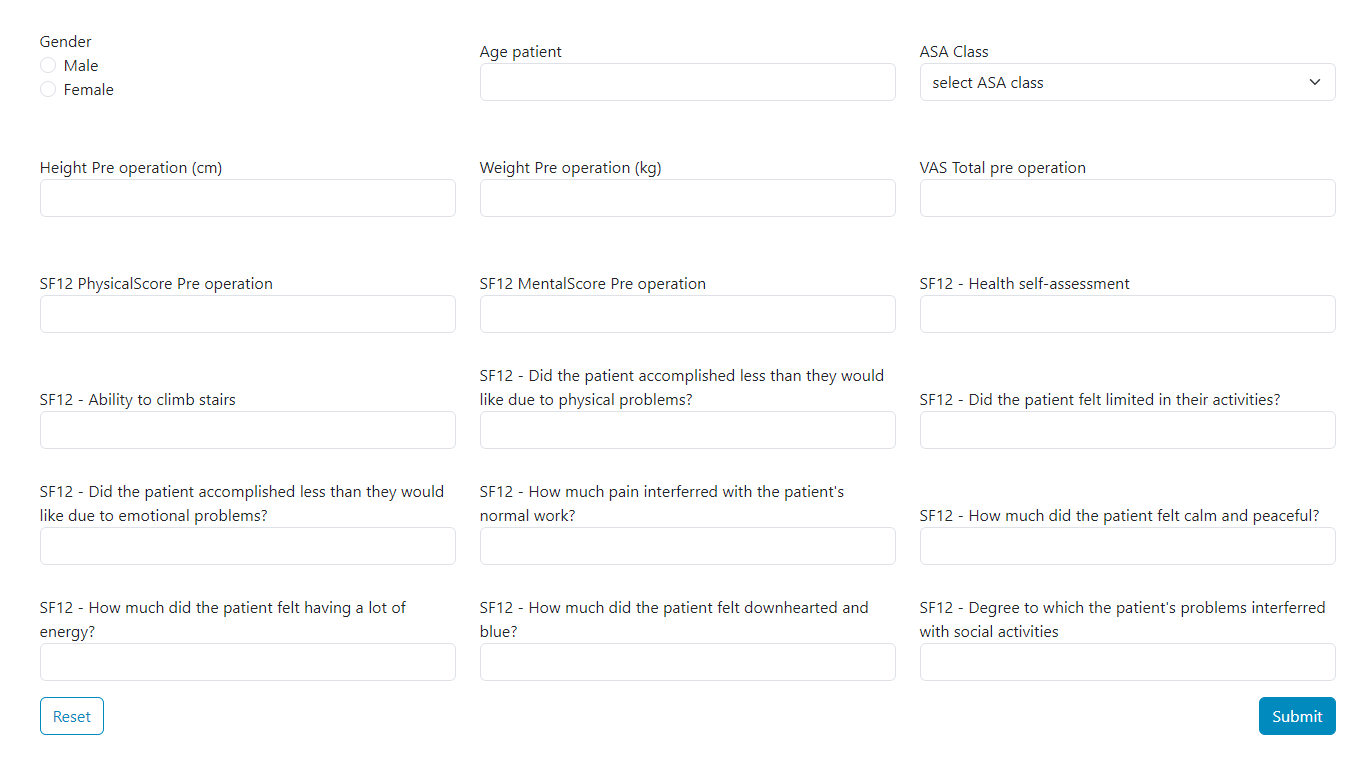
\includegraphics[width=0.9\columnwidth]{epimetheus-questionario-paziente} 
    \caption{Questionario presente nella pagina inziaile di Epimetheus}
\end{figure}